\chapter{Evaluation}
\section{Experiments and Measurements}
\subsection{Experiment A: Orchestral Concert to Analyze Musical Absorption using Nidra to Collect Breathing Data}
The experiment was conducted in collaboration with master student Joachim Dalgard at the University of Oslo at the faculty of \textit{RITMO: Centre for Interdisciplinary Studies in Rhythm, Time and Motion}. 

The goal of the experiment was to analyze musical absorption, which is a state an individuals ability and willingness allows music to draw them into an emotional experience and becomes unaware of time and space. In order to analyze the effect of musical absorption on individuals, we gathered 20 participants who were experienced listeners with musical education. The participants attended an orchestral concert by Richard Strauss' Alpine Symphony---a symphonic poem that portrays the experience of eleven hours spent climbing an Alpine mountain---that lasted around 50 minutes at Oslo Concert Hall on third of April and fourth of April 2019.  

The participants were divided into two groups to attend the concert on the two dates. Each participant was equipped with a wireless electromyographic sensor from DELSYS in order to measure heart rate, and a Flow sensor kit to measure respiration during the concert. RITMO had multiple Flow sensors for disposal; however, they had no suitable mobile application that could record with these sensors. Also, with their equipment they experienced that Flow sensor kits had a tendency to disconnect every 10-15 minutes, resulting in fragmented recordings for a single session. Therefore, they reached out to \textit{Insitute for Informatics} in hopes of a solution. Our application was a suiting match for both parties, hence a collaboration was formed. We arranged for six Android devices and reached out to the participants to bring their Android devices if they had one. There were ten participants in each group and six assessed devices. As a precaution, we decided to give out the devices to the participants who scored highest on a test performed on beforehand.

The motivation for this experiment in regards to Nidra was to test the application in a real-life and crowded environment. During the concert, there were approximately 800 attendees on the first day and approximately 1500 attendees on the second day. We can assume that most of the attendees had a mobile device, and a few shares of them had BlueTooth activated on the device. Based on these estimates, we were able to replicate an environment (on a larger scale) where other devices might interfere with the signals between the collecting sensor and the application. Also, we were able to install the application on multiple mobile devices with different Android OS versions and put the application in the hands of the participants. 

\subsubsection{Preperations}

\begin{table}
\begin{center}
\scalebox{0.59}{
\begin{tabular}{ |c|c|c|c| } 
\hline
\textbf{Model} & \textbf{Samsung Galaxy S9} & \textbf{OnePlus 3T} & \textbf{Google Pixel XL} \\
\hline
Operating System & Android 8.0 & - & Android 9.0 \& Android 7.1.2  \\
Chipset & Exynos 9810  & Qualcomm MSM8996 Snapdragon 821 & Qualcomm MSM8996 Snapdragon 821  \\
CPU & Octa-core & Quad-core & Quad-core \\
GPU & Mali-G72 MP18 & Adreno 530 & Adreno 530  \\
RAM & 4 GB & 6 GB & 4 GB \\
Battery & Li-Ion 3000 mAh & Li-Ion 3400 mAh & Li-Ion 3450 mAh  \\
Bluetooth & 5.0, A2DP, LE, aptX & 4.2, A2DP, aptX HD, LE & 4.2, A2DP, LE, aptX \\

\hline
\end{tabular}}
\caption{Device models used during the concert}
\end{center}
\end{table}

In order to partake in the experiments, we had to ensure that the mobile devices were configured correctly. Also, stress testing the application to prevent ... 

\begin{description}
    \item[Device Configuration] The device models in our disposal had to be configured with the applications to enable recording on Nidra. First, the data stream dispatching module had to be installed on the devices. Second, the sensor wrapper for the Flow sensor kit had to be configured with the respective sensor (in order to reduce the time on setup the sensor and application to the participant). Lastly, the Nidra application had be to initiated with appropritately user information, in order to distingish each participants with the sensor and device model. In Figure 6.1, the device models are listed with their spesifications, and the OS ...
    \item[Obsticle] One of the pressing concerns at the time of the experiment was to ensure a persistent connection between the sensor and application---uninterrupted by sensor disconnections and disruptions---in order to collect meaningful data.  At the time of development, there was no mechanism to reconnect with the sensors on disconnect or disruption during recording. Therefore, the mechanism had to be developed, otherwise, the recording would not be able to capture the respiration of the participant through the whole concert. 
    \item[Body Placement] The respiration value is based on the participant body circumference and changes are assosicated with breathing. The participant was instructed to place the sensor around their thorax (just below the armpits), in order to measure the expansion and contraction of the rib cage, to measure the respiration flow. Also, the respiration can vary through the recording based on body position (e.g., sitting relax or tense in a chair). 

\end{description}


\subsubsection{Results}

We had thirteen mobile devices combined for the both dates---the extra device was from one of the participents---however, the application crashed on one of the mobile devices during the recording, rendering  in an incomplete recording on one of the mobile devices. Therefore, we have access to tvelwe recordings from the concerts. Figure \ref{fig:day_1} and Figure \ref{fig:day_2} present two of these tvelwe recordings (rest can be found in Appendix B) in a time-series graph that are of most interest to us. The Y-axis presents the respiration (breathing) value, and the X-axis the time of respiration value acqusition---day 1 of the concert started at time of 19:00 and ended at 20:00, while day 2 started at time of 20:10 and ended 21:00. The graphs are plotted with Python and the library MatPlotLib in order to analyse and evaluation the graphs; however, an identical graph is also presented in the application.

\begin{figure}
\parbox{7cm}{
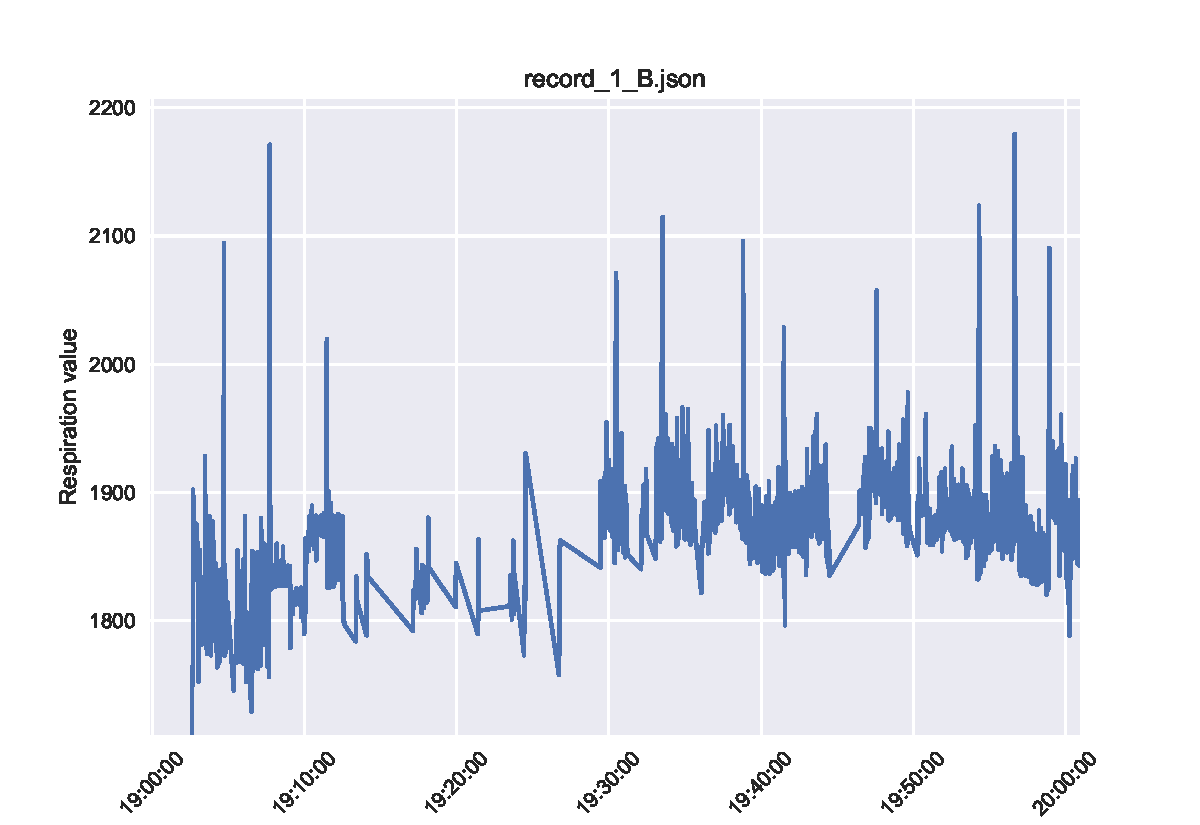
\includegraphics[width=8cm]{images/Record_1_B.pdf}
\caption{Concert Day 1---Mobile Device B}
\label{fig:day_1}}
\qquad
\begin{minipage}{6cm}
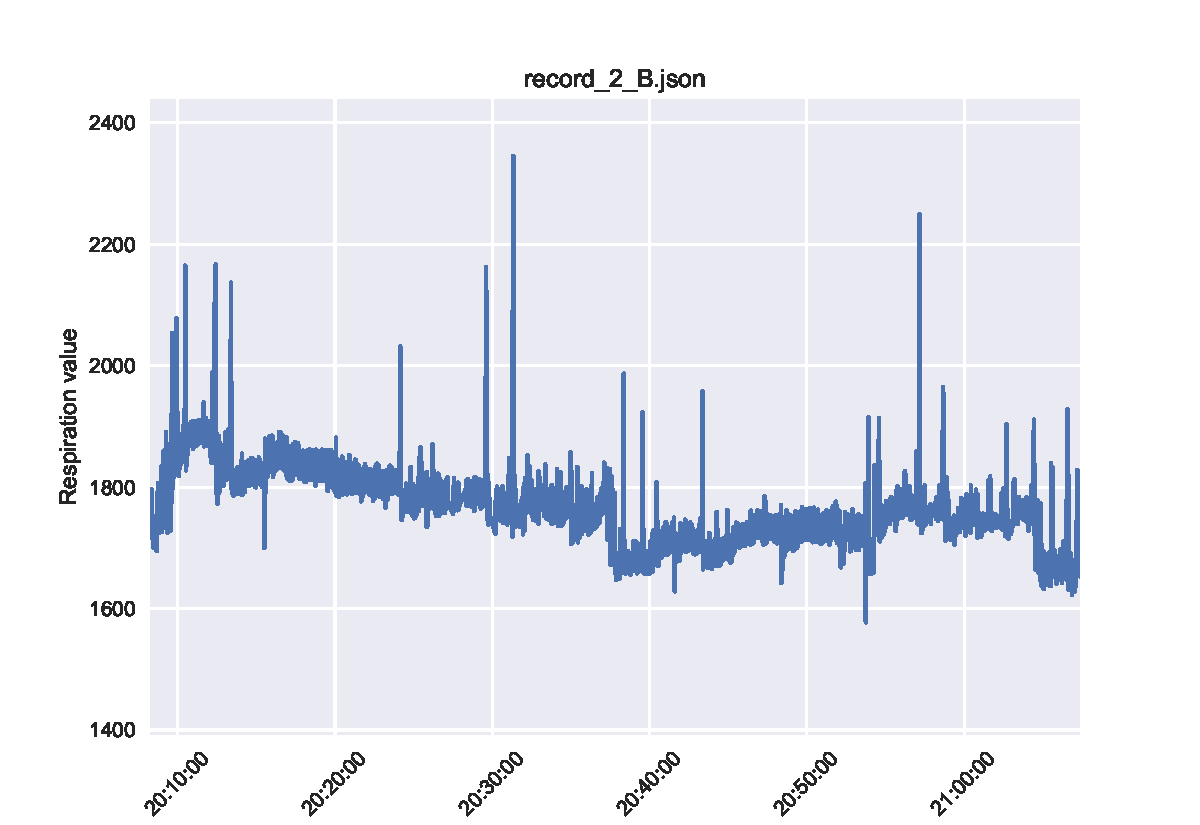
\includegraphics[width=7cm]{images/Record_2_B.pdf}
\caption{Concert Day 2---Mobile Device B}
\label{fig:day_2}
\end{minipage}
\end{figure}

\subsubsection{Analysis \& Discussion}
To begin with, we will investigate all of recordings by analyzing the respiration values. We are specially interested in finding occourances of disconnects---when the samples are stagnant in longer period, in contrasts to spikes which emulates breathing by contraction and extraction of the body---and the time it takes the application to reconnect with the sensor.


\begin{table}
\begin{center}
\scalebox{0.7}{
\begin{tabular}{ |c|c|c|c||c|c| } 
\hline
\textbf{Model} & \textbf{Samples} & \textbf{Loss Count} & \textbf{Loss Percentage} & \textbf{Times Disconnected} & \textbf{Time Disconnected} \\
\hline
A & 5145 & 0 & 0 \% & 0  & 00:00  \\
\hline
B & 3363 & 1782 & 34 \% & 13 & 19m:14s  \\
\hline
C & 4189 & 956 & 19 \% & 7 & 8m:20s  \\
\hline
D & 3501 & 1644 & 32 \% & 5 & 18m:30s  \\
\hline
E & 5144 & 1 & 0.02 \% & - & -  \\
\hline
F & 5145 & 0  & 0 \% & 0 & 00:00  \\
\hline
\end{tabular}}
\caption{Day 1---Duration: 1 hour \& Roof Samples: 5145}
\end{center}
\end{table}


\begin{table}
\begin{center}
\scalebox{0.7}{
\begin{tabular}{ |c|c|c|c||c|c| } 
\hline
\textbf{Model} & \textbf{Samples} & \textbf{Loss Count} & \textbf{Loss Percentage} & \textbf{Times Disconnected} & \textbf{Time Disconnected} \\
\hline
A & 4286 & 2 & 0.05 \% & -  & -  \\
\hline
B & 4161 & 127 & 3 \% & 4 & 1m:25s  \\
\hline
C & 4286 & 2 & 0.05 \% & - & -  \\
\hline
D & 2576 & 1712 & 40 \% & 7 & 24m:35s  \\
\hline
E & 4285 & 3 & 0.06 \% & - & -  \\
\hline
F & 4288 & 0  & 0 \% & 0 & 00:00  \\
\hline
\end{tabular}}
\caption{Day 2---Duration: 50 mins. \& Roof Samples: 4288}
\end{center}
\end{table}


To conclude this experiment, 

\subsection{Experiment B: 8-hours recording}
\subsection{Experiment C: User-Experience}

\subsection{Experiment D: Creating a Simple Module}



\section{Main Findings}
